\chapter{Anleitung}
\label{Anleitung}

\section{Konfiguration}
In der Konfiguration kann man verschiedene Einstellungen für das Verhalten des Spiels vornehmen.

\begin{figure}[h]
  \begin{center}
    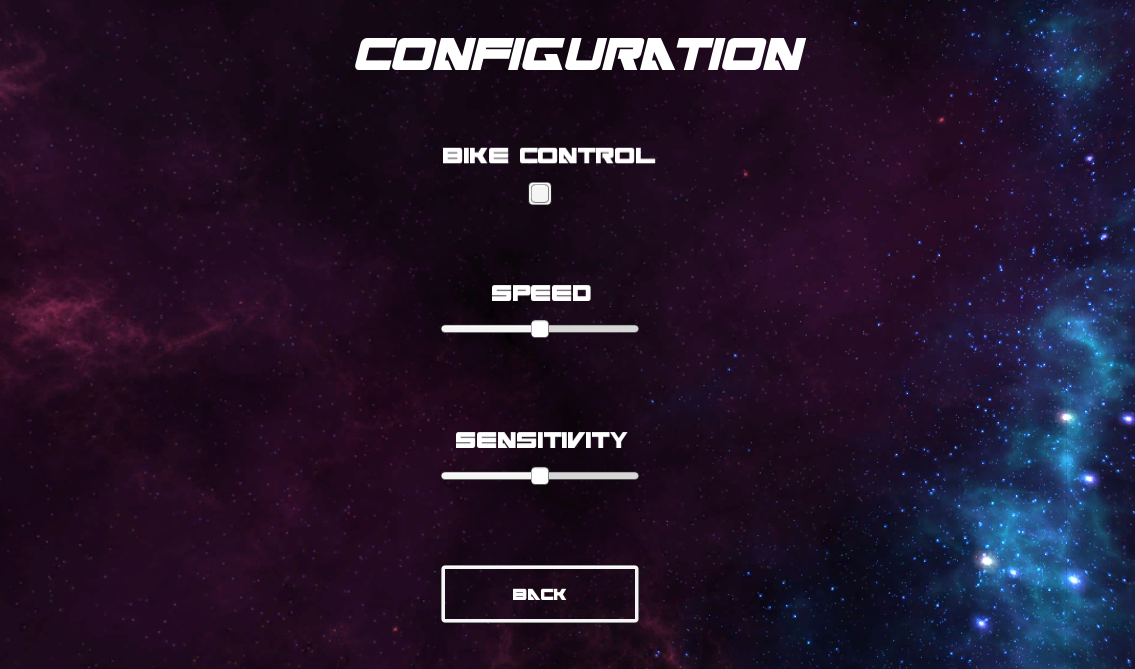
\includegraphics[width=.9\textwidth]{gfx/anleitung/config.png}
    \caption{Konfiguration}
  \end{center}
\end{figure}

\begin{itemize}
  \item \textbf{Bike Controls} \\
  Ist diese Option ausgewählt, kann das Spiel mit Hilfe des Ergometers gesteuert werden, anderenfalls steuert man das Raumschiff mit den Pfeiltasten auf der Tastatur, sowie der Leertaste.
  \item \textbf{Speed} \\
  Diese Option bietet die Möglichkeit die Geschwindigkeit des Ergometers anzupassen. Standardmäßig befindet sich der Geschwindigkeitsmodifikator auf einem mittleren Wert. Um die Geschwindigkeit anzupassen kann der Wert entweder verringert oder erhöht werden. Ein höherer Wert des Reglers bedeutet eine schnellere Geschwindigkeit, ein niedriger Wert entsprechend eine langsamere Geschwindigkeit.
  \item \textbf{Sensitivity}\\
   Diese Option beeinflusst, ähnlich wie die Geschwindigkeit, die Sensitivität des Ergometers. Je nach Einstellung des Reglers reagiert das Fahrrad leichter oder schwerer. Wird der Regler auf einen hohen Wert eingestellt reagiert das Ergometer mehr auf Veränderungen der Neigung. Ein niedriger Wert senkt die Sensitivität entsprechend.
  \item \textbf{Back} \\
  Durch drücken des Buttons \textit{Back} werden die Einstellungen gespeichert und man gelangt ins Hauptmenü zurück.
\end{itemize}

\section{Steuerung}
Das Spiel besitzt zwei Möglichkeiten der Steuerung: Tastatur- und Ergometersteuerung. Bei beiden Varianten kann jeweils zusätzlich die Maus genutzt werden. \\

\subsection{Tastatursteuerung}
Ist in der Konfiguration nicht die Steuerung mittels Ergometer aktiviert gilt folgende Tastenbelegung.

\begin{itemize}
  \item \textbf{Pfeiltaste Hoch:} Erhöht die Geschwindigkeit des Raumschiffes.
  \item \textbf{Pfeiltaste Runter:} Verringert die Geschwindigkeit des Raumschiffes.
  \item \textbf{Pfeiltasten Links/Rechts:} Steuerung des Raumschiffes nach Links oder Rechts.
  \item \textbf{Leertaste:} Lässt das Raumschiff springen.
  \item \textbf{Rechte Maustaste:} Neustart des aktuellen Levels
  \item \textbf{Escape:} Zurück zum Hauptmenü.
\end{itemize}

\subsection{Ergometersteuerung}
Ist die Ergometersteuerung eingeschaltet gibt es folgende Eingabemöglichkeiten.

\begin{itemize}
  \item \textbf{Trittfrequenz erhöhen:} Erhöht die Geschwindigkeit des Raumschiffs.
  \item \textbf{Trittfrequenz verringern:} Verringert die Geschwindigkeit des Raumschiffes.
  \item \textbf{Neigung des Ergometers nach Links/Rechts:} Steuerung des Raumschiffes nach Links oder Rechts.
  \item \textbf{Linke Maustaste:} Lässt das Raumschiff springen.
  \item \textbf{Rechte Maustaste:} Neustart des aktuellen Levels
  \item \textbf{Escape:} Zurück zum Hauptmenü.
\end{itemize}

\section{Spiel}
Hat der Benutzer das eigentliche Spiel gestartet findet er diverse Informationen vor, die ihm ein Feedback über den aktuellen Status des Spiels vermitteln sollen. Die einzelnen Objekte und Anzeigen werden nachfolgend erläutert.

\begin{enumerate}
  \item \textbf{Levelanzeige} \\
   Diese Anzeige zeigt die Nummer des aktuellen Levels an.
  \item \textbf{Fortschrittsanzeige} \\
  Hier wird der Fortschritt im akutellen Level angezeigt. Je voller der Balken ist, desto weiter fortgeschritten ist der Spieler.
  \item \textbf{Spielfigur} \\
  Die durch den Spieler gesteuerte Figur. Die Düsenantriebe geben zusätzlich ein Feedback über die aktuelle Geschwindigkeit.
  \item \textbf{Kraftstoffanzeige}\\
  Hier erkennt der Spieler den verbleibenden Kraftstoff. Verbleibender Kraftstoff symbolisiert die Zeit, die dem Spieler bleibt das Level zu beenden. Je voller der Kreis ist, desto mehr Kraftstoff verbleibt dem Spieler. Ist der Kraftstoff aufgebraucht gilt das Level als verloren und der Spieler muss das Level von Vorne beginnen. Das Raumschiff beginnt Kraftstoff zu verbrauchen, sobald es zum ersten mal beschleunigt wird.
  \item \textbf{Geschwindigkeitsanzeige}\\
  Zeigt die aktuelle Geschwindigkeit an. Befindet sich das Raumschiff im Stillstand ist die Anzeige leer, hat der Spieler die maximale Geschwindigkeit erreicht ist die anzeige komplett gefüllt. 
  \item \textbf{Bahn} \\
  Die Bahn ist das eigentliche Level. Der Spieler darf nicht von ihr abkommen, sonst muss er das Level neu beginnen. Am Ende der Bahn befindet sich ein Zielbereich. Erreicht er das Ziel bevor ihm der Treibstoff ausgeht hat er das Level erfolgreich beendet. Die Bahn kann neben der normalen Fahrbahn aus verschiedenen Objekten und Hindernissen bestehen. Beispiele hierfür sind Tunnel, Rampen oder verschiedene Blöcke, die in späteren Leveln nach und nach eingeführt werden.
\end{enumerate}

\begin{figure}
  \begin{center}
    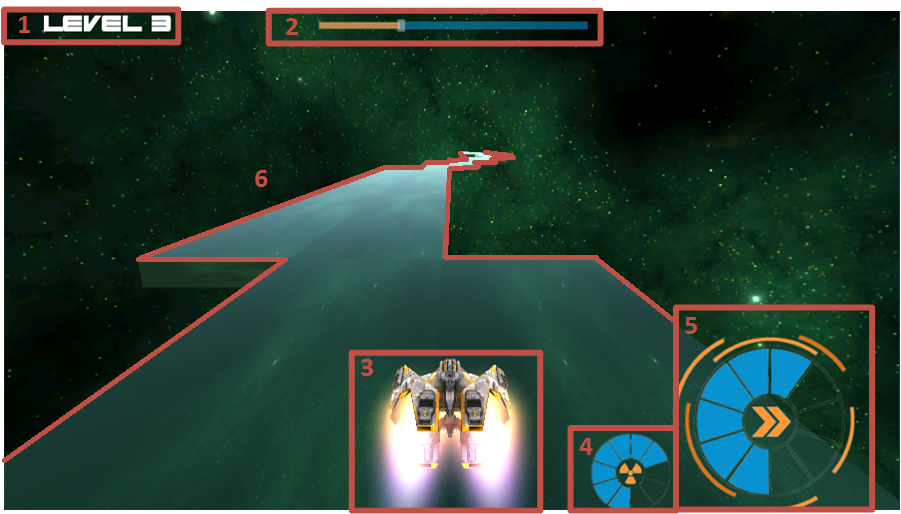
\includegraphics[width=.9\textwidth]{gfx/anleitung/ingame2.png}
    \caption{Spielansicht}
  \end{center}
\end{figure}
